\setcounter{ex}{0}
\setcounter{dang}{0}
\section{Mức 5,6 điểm}
\begin{dang}{Tìm khoảng đơn điệu của hàm số thông qua bảng biến thiên, đồ thị}	
\end{dang}
\Opensolutionfile{ans}[ans/CD1/Muc_5_6]
\begin{ex}%[Phạm Hoàng Điệp]%[2D1Y1-2]%Câu 1
	[Mã 101 – 2020 Lần 1] Cho hàm số $f(x)$ có bảng biến thiên như sau:
	\begin{center}
		\begin{tikzpicture}[>=stealth]
			\tkzTabInit[nocadre,lgt=1.2,espcl=2,deltacl=0.5]{$x$/.7 ,$f'(x)$/.7,$f(x)$/2}
			{$-\infty$ , $-1$ , $0$ , $1$ , $+\infty$}
			\tkzTabLine{ , - , $0$ , + , $0$ , - , $0$ , + , }
			\tkzTabVar{+/$+\infty$ , -/$-1$, +/$4$ , -/$-1$ , +/$+\infty$}
		\end{tikzpicture}
	\end{center}
	Hàm số đã cho đồng biến trên khoảng nào dưới đây?
	\choice
	{$\left(-\infty ;-1\right)$}
	{$\left(0;1\right)$}
	{$\left(-1;1\right)$}
	{\True $\left(-1;0\right)$}
	\loigiai{
		Hàm số đã cho đồng biến trên khoảng $\left(-1;0\right)$ và $\left(1;+\infty\right)$.}
\end{ex}

\begin{ex}%[Phạm Hoàng Điệp]%[2D1Y1-2]%Câu 2
	[Mã 103-2019] Cho hàm số $f(x)$ có bảng biến thiên như sau:
	\begin{center}
		\begin{tikzpicture}[>=stealth]
			\tkzTabInit[nocadre,lgt=1.2,espcl=2,deltacl=0.5]{$x$/.7 ,$f'(x)$/.7,$f(x)$/2}
			{$-\infty$ , $-1$ , $0$ , $1$ , $+\infty$}
			\tkzTabLine{ , - , $0$ , + , $0$ , - , $0$ , + , }
			\tkzTabVar{+/$+\infty$ , -/$0$, +/$3$ , -/$0$ , +/$+\infty$}
		\end{tikzpicture}
	\end{center}
	Hàm số đã cho đồng biến trên khoảng nào sau đây?
	\choice
	{$\left(-\infty ;-1\right)$}
	{$ \left(0;1\right) $}
	{\True $\left(-1;0\right)$}
	{$\left(-1;+\infty\right)$}
	\loigiai{
		Hàm số đã cho đồng biến trên khoảng $\left(-1;0\right).$}
\end{ex}

\begin{ex}%[Phạm Hoàng Điệp]%[2D1Y1-2]%Câu 3
	[Mã 104-2017] Cho hàm số $y=f(x)$ có bảng xét dấu đạo hàm như sau
	\begin{center}
		% Cần khai báo \usepackage{tkz-tab}
		\begin{tikzpicture}
			\tkzTabInit[nocadre,lgt=2,espcl=2,deltacl=0.5]{$x$/1 ,$f'(x)$/1}
			{$-\infty$ , $-2$ , $0$ , $2$ , $+\infty$}
			\tkzTabLine{  , + , 0 , - , d , - , 0 , + }
		\end{tikzpicture}	
	\end{center}
	Mệnh đề nào dưới đây đúng?
	\choice
	{Hàm số nghịch biến trên khoảng $\left(-\infty ;-2\right)$}
	{Hàm số đồng biến trên khoảng $\left(-2;0\right)$}
	{Hàm số đồng biến trên khoảng $\left(-\infty ;0\right)$}
	{\True Hàm số nghịch biến trên khoảng $\left(0;2\right)$}
	\loigiai{
		Theo bảng xét dấu thì $y'<0$ khi $x\in(0;2)$ nên hàm số nghịch biến trên khoảng $(0;2)$.}
\end{ex}

\begin{ex}%[Phạm Hoàng Điệp]%[2D1Y1-2]%Câu 4
	[Kim Liên-Hà Nội-2019] Cho hàm số $y=f(x)$ có bảng xét dấu của đạo hàm như hình vẽ. Hàm số đã cho nghịch biến trên khoảng nào dưới đây?
	\begin{center}
		\begin{tikzpicture}
			\tkzTabInit[nocadre,lgt=2,espcl=2,deltacl=0.5]{$x$/1 ,$f'(x)$/1}
			{$-\infty$ , $-1$ , $1$ , $+\infty$}
			\tkzTabLine{  , - , d , - , 0 , + , }
		\end{tikzpicture}
	\end{center}
	\choice
	{$\left(1;+\infty\right)$}
	{$\left(-\infty;1\right)$}
	{$\left(-1;+\infty\right)$}
	{\True $\left(-\infty;-1\right)$}
	\loigiai
	{Từ bảng xét dấu ta thấy hàm số đã cho nghịch biến trên khoảng $\left(-\infty;-1\right)$ và $\left(-1;1\right)$.\\
		Vậy hàm số đã cho nghịch biến trên khoảng $\left(-\infty;-1\right)$.}
\end{ex}

\begin{ex}%[Phạm Hoàng Điệp]%[2D1Y1-2]%Câu 5
	[Mã 101-2018] Cho hàm số$y=f(x)$ có bảng biến thiên như sau
	\begin{center}
		\begin{tikzpicture}[>=stealth]
			\tkzTabInit[nocadre,lgt=1.2,espcl=2,deltacl=0.5]{$x$/.7 ,$f'(x)$/.7,$f(x)$/2}
			{$-\infty$ , $-1$ , $0$ , $1$ , $+\infty$}
			\tkzTabLine{ , - , $0$ , + , $0$ , - , $0$ , + , }
			\tkzTabVar{+/$+\infty$ , -/$-2$, +/$3$ , -/$-2$ , +/$+\infty$}
		\end{tikzpicture}
	\end{center}
	Hàm số đã cho nghịch biến trên khoảng nào dưới đây?
	\choice
	{$\left(-1;0\right)$}
	{$\left(-\infty ;0\right)$}
	{$\left(1;+\infty\right)$}
	{\True $\left(0;1\right)$}
	\loigiai{
		Dựa vào bảng biến thiên ta có hàm số đã cho nghịch biến trên các khoảng $\left(0;1\right)$ và $\left(-\infty ;-1\right)$.}
\end{ex}

\begin{ex}%[Phạm Hoàng Điệp]%[2D1Y1-2]%Câu 6
	[Mã 102-2019] Cho hàm số $f(x)$ có bảng biến thiên như sau:
	\begin{center}
		\begin{tikzpicture}[>=stealth]
			\tkzTabInit[nocadre,lgt=1.2,espcl=2,deltacl=0.5]{$x$/.7 ,$f'(x)$/.7,$f(x)$/2}
			{$-\infty$ , $-2$ , $0$ , $2$ , $+\infty$}
			\tkzTabLine{ , - , $0$ , + , $0$ , - , $0$ , + , }
			\tkzTabVar{+/$+\infty$ , -/$1$, +/$3$ , -/$1$ , +/$+\infty$}
		\end{tikzpicture}
	\end{center}
	Hàm số đã cho đồng biến trên khoảng nào dưới đây?
	\choice
	{$\left(0;+\infty\right)$}
	{$\left(0;2\right)$}
	{\True $\left(-2;0\right)$}
	{$\left(-\infty ;-2\right)$}
	\loigiai{
		Từ bảng biến thiên, suy ra trên khoảng $\left(-2;0\right)$ hàm số đồng biến.}
\end{ex}

\begin{ex}%[Phạm Hoàng Điệp]%[2D1Y1-2]%Câu 7
	[Mã 103-2018] Cho hàm số $y=f(x)$ có bảng biến thiên như sau:
	\begin{center}
		\begin{tikzpicture}[>=stealth]
			\tkzTabInit[nocadre,lgt=1.2,espcl=2,deltacl=0.5]{$x$/.7 ,$f'(x)$/.7,$f(x)$/2}
			{$-\infty$ , $-1$ , $0$ , $1$ , $+\infty$}
			\tkzTabLine{ , + , $0$ , - , $0$ , + , $0$ , - , }
			\tkzTabVar{-/$-\infty$ , +/$-1$, -/$-2$ , +/$-1$ , -/$-\infty$}
		\end{tikzpicture}
	\end{center}
	Hàm số đã cho đồng biến trên khoảng nào dưới đây?
	\choice
	{\True $\left(0;1\right)$}
	{$\left(1;+\infty\right)$}
	{$\left(-\infty ;1\right)$}
	{$\left(-1;0\right)$}
	\loigiai{
	}
\end{ex}

\begin{ex}%[Phạm Hoàng Điệp]%[2D1Y1-2]%Câu 8
	[Mã 101-2019] Cho hàm số có bảng biến thiên như sau
	\begin{center}
		\begin{tikzpicture}[>=stealth]
			\tkzTabInit[nocadre,lgt=1.2,espcl=2,deltacl=0.5]{$x$/.7 ,$f'(x)$/.7,$f(x)$/2}
			{$-\infty$ , $-2$ , $0$ , $2$ , $+\infty$}
			\tkzTabLine{ , - , $0$ , + , $0$ , - , $0$ , + , }
			\tkzTabVar{+/$+\infty$ , -/$1$, +/$3$ , -/$1$ , +/$+\infty$}
		\end{tikzpicture}
	\end{center}
	Hàm số đã cho nghịch biến trên khoảng nào dưới đây?
	\choice
	{\True $\left(0;2\right)$}
	{$\left(0;+\infty\right)$}
	{$\left(-2;0\right)$}
	{$\left(2;+\infty\right)$}
	\loigiai{
		Dựa vào bảng biến thiên ta thấy trên khoảng $\left(0;2\right)$ thì $f'(x)<0$.\\
		Vậy hàm số nghịch biến trên khoảng $\left(0;2\right)$.}
\end{ex}

\begin{ex}%[Phạm Hoàng Điệp]%[2D1Y1-2]%Câu 9
	[Mã 102-2018] Cho hàm số $y=f(x)$ có bảng biến thiên như sau:
	\begin{center}
		\begin{tikzpicture}[>=stealth]
			\tkzTabInit[nocadre,lgt=1.2,espcl=2,deltacl=0.5]{$x$/.7 ,$f'(x)$/.7,$f(x)$/2}
			{$-\infty$ , $-1$ , $1$ , $+\infty$}
			\tkzTabLine{ , + , $0$ , - , $0$ , + , }
			\tkzTabVar{-/$-\infty$ , +/$3$ , -/$-2$ , +/$+\infty$}
		\end{tikzpicture}
	\end{center}
	Hàm số đã cho đồng biến trên khoảng nào dưới đây?
	\choice
	{$\left(-1;+\infty\right)$}
	{\True $\left(1;+\infty\right)$}
	{$\left(-1;1\right)$}
	{$\left(-\infty ;1\right)$}
	\loigiai{
		
	}
\end{ex}

\begin{ex}%[Phạm Hoàng Điệp]%[2D1Y1-2]%Câu 10
	[Mã 104-2018] Cho hàm số $y=f(x)$ có bảng biến thiên như sau
	\begin{center}
		\begin{tikzpicture}[>=stealth]
			\tkzTabInit[nocadre,lgt=1.2,espcl=2,deltacl=0.5]{$x$/.7 ,$f'(x)$/.7,$f(x)$/2}
			{$-\infty$ , $-2$ , $3$ , $+\infty$}
			\tkzTabLine{ , - , $0$ , + , $0$ , - , }
			\tkzTabVar{+/$+\infty$ , -/$1$ , +/$4$ , -/$-\infty$}
		\end{tikzpicture}
	\end{center}
	Hàm số đã cho đồng biến trên khoảng nào dưới đây?
	\choice
	{\True $\left(-2;3\right)$}
	{$\left(3;+\infty\right)$}
	{$\left(-\infty ;-2\right)$}
	{$\left(-2;+\infty\right)$}
	\loigiai{}
\end{ex}

\begin{ex}%[Phạm Hoàng Điệp]%[2D1Y1-2]%Câu 11
	[Đề Tham Khảo 2018] Cho hàm số $y=f(x)$ có bảng biến thiên như sau:
	\begin{center}
		\begin{tikzpicture}[>=stealth]
			\tkzTabInit[nocadre,lgt=1.2,espcl=2,deltacl=0.5]{$x$/.7 ,$f'(x)$/.7,$f(x)$/2}
			{$-\infty$ , $-2$ , $0$ , $2$ , $+\infty$}
			\tkzTabLine{ , + , $0$ , - , $0$ , + , $0$ , - , }
			\tkzTabVar{-/$-\infty$ , +/$3$, -/$-1$ , +/$3$ , -/$-\infty$}
		\end{tikzpicture}
	\end{center}
	Hàm số $y=f(x)$ nghịch biến trên khoảng nào dưới đây?
	\choice
	{$\left(0;+\infty\right)$}
	{$\left(-\infty ;-2\right)$}
	{$\left(0;2\right)$}
	{\True $\left(-2;0\right)$}
	\loigiai{
		Hàm số $y=f(x)$ nghịch biến trên khoảng $\left(-2;0\right)$.
	}
\end{ex}

\begin{ex}%[Phạm Hoàng Điệp]%[2D1Y1-2]%Câu 12
	[Đề Minh Họa 2020 – Lần 1] Cho hàm số $f(x)$ có bảng biến thiên như sau:
	\begin{center}
		\begin{tikzpicture}[>=stealth]
			\tkzTabInit[nocadre,lgt=1.2,espcl=2,deltacl=0.5]{$x$/.7 ,$f'(x)$/.7,$f(x)$/2}
			{$-\infty$ , $-1$ , $0$ , $1$ , $+\infty$}
			\tkzTabLine{ , + , $0$ , - , $0$ , + , $0$ , - , }
			\tkzTabVar{-/$-\infty$ , +/$2$, -/$-1$ , +/$2$ , -/$-\infty$}
		\end{tikzpicture}
	\end{center}
	Hàm số đã cho nghịch biến trên khoảng nào dưới đây?
	\choice
	{$\left(-\infty ;-1\right)$}
	{$\left(0;1\right)$}
	{\True $\left(-1;0\right)$}
	{$\left(-\infty ;0\right)$}
	\loigiai{}
\end{ex}

\begin{ex}%[Phạm Hoàng Điệp]%[2D1Y1-2]%Câu 13
	[Đề Minh Họa 2020 – Lần 2] Cho hàm số $y=f(x)$ có bảng biến thiên như sau
	\begin{center}
		\begin{tikzpicture}[>=stealth]
			\tkzTabInit[nocadre,lgt=1.2,espcl=2,deltacl=0.5]{$x$/.7 ,$f'(x)$/.7,$f(x)$/2}
			{$-\infty$ , $-2$ , $0$ , $2$ , $+\infty$}
			\tkzTabLine{ , + , $0$ , - , $0$ , + , $0$ , - , }
			\tkzTabVar{-/$-\infty$ , +/$2$, -/$-1$ , +/$2$ , -/$-\infty$}
		\end{tikzpicture}
	\end{center}
	Hàm số đã cho đồng biến trên khoảng nào dưới đây?
	\choice
	{$\left(1;+\infty\right)$}
	{$\left(-1;0\right)$}
	{$\left(-1;1\right)$}
	{\True $\left(0;1\right)$}
	\loigiai{
		Dựa vào bảng biến thiên ta thấy: Hàm số đã cho đồng biến trên các khoảng $\left(-\infty;-1\right)$ và $\left(0;1\right)$.}
\end{ex}

\begin{ex}%[Phạm Hoàng Điệp]%[2D1Y1-2]%Câu 14
	[Mã 102 – 2020 Lần 1] Cho hàm số $ f(x) $ có bảng biến thiên như sau.
	\begin{center}
		\begin{tikzpicture}[>=stealth]
			\tkzTabInit[nocadre,lgt=1.2,espcl=2,deltacl=0.5]{$x$/.7 ,$f'(x)$/.7,$f(x)$/2}
			{$-\infty$ , $-1$ , $0$ , $1$ , $+\infty$}
			\tkzTabLine{ , + , $0$ , - , $0$ , + , $0$ , - , }
			\tkzTabVar{-/$-\infty$ , +/$4$, -/$1$ , +/$4$ , -/$-\infty$}
		\end{tikzpicture}
	\end{center}
	Hàm số đã cho đồng biến trên khoảng nào dưới đây?
	\choice
	{$ (1;+\infty) $}
	{$ (-1;1) $}
	{\True $ (0;1) $}
	{$ (-1;0) $}
	\loigiai{
		Dựa vào bảng biến thiên, ta thấy hàm số đã cho đồng biến trên các khoảng $ (-\infty;-1) $ và $ (0;1) $.
	}
\end{ex}

\begin{ex}%[Phạm Hoàng Điệp]%[2D1Y1-2]%Câu 15
	[Mã 103 – 2020 Lần 1] Cho hàm số $f(x)$ có bảng biến thiên như sau:
	\begin{center}
		\begin{tikzpicture}[>=stealth]
			\tkzTabInit[nocadre,lgt=1.2,espcl=2,deltacl=0.5]{$x$/.7 ,$f'(x)$/.7,$f(x)$/2}
			{$-\infty$ , $-2$ , $0$ , $2$ , $+\infty$}
			\tkzTabLine{ , + , $0$ , - , $0$ , + , $0$ , - , }
			\tkzTabVar{-/$-\infty$ , +/$3$, -/$2$ , +/$3$ , -/$-\infty$}
		\end{tikzpicture}
	\end{center}
	Hàm số đã cho đồng biến trên khoảng nào dưới đây
	\choice
	{$(-2;2)$}
	{\True $(0;2)$}
	{$(-2;0)$}
	{$(2;+\infty)$}
	\loigiai{}
\end{ex}

\begin{ex}%[Phạm Hoàng Điệp]%[2D1Y1-2]%Câu 16
	[Mã 104 – 2020 Lần 1] Cho hàm số $f(x)$ có bảng biến thiên như sau:
	\begin{center}
		\begin{tikzpicture}[>=stealth]
			\tkzTabInit[nocadre,lgt=1.2,espcl=2,deltacl=0.5]{$x$/.7 ,$f'(x)$/.7,$f(x)$/2.5}
			{$-\infty$ , $-3$ , $0$ , $3$ , $+\infty$}
			\tkzTabLine{ , - , $0$ , + , $0$ , - , $0$ , + , }
			\tkzTabVar{+/$+\infty$ , -/$-1$, +/$1$ , -/$-1$ , +/$+\infty$}
		\end{tikzpicture}
	\end{center}
	Hàm số đã cho đồng biến trên khoảng nào dưới đây?
	\choice
	{\True $\left(-3;0\right)$}
	{$\left(-3;3\right)$}
	{$\left(0;3\right)$}
	{$\left(-\infty ;-3\right)$}
	\loigiai{
		Hàm số đã cho đồng biến trên khoảng $\left(-3;0\right)$ và $\left(3;+\infty\right)$.}
\end{ex}

\begin{ex}%[Phạm Hoàng Điệp]%[2D1Y1-2]%Câu 17
	Cho hàm số $y=f(x)$ có bảng biến thiên như hình dưới đây. Mệnh đề nào sau đây là đúng?
	\begin{center}
		\begin{tikzpicture}[>=stealth]
			\tkzTabInit[nocadre,lgt=1.2,espcl=2.2,deltacl=0.7]{$x$/1 ,$f'(x)$/.7,$f(x)$/2.5}
			{ $-\infty$ , $-\dfrac{1}{2}$ , $3$ , $+\infty$}
			\tkzTabLine{, + , d , + , $0$ , - , }
			\tkzTabVar{-/$-\infty$ , +D-/$+\infty$/$-\infty$ , +/$4$ , -/$-\infty$}
		\end{tikzpicture}
	\end{center}
	\choice
	{Hàm số đã cho đồng biến trên khoảng $\left(-\dfrac{1}{2};+\infty\right)$}
	{Hàm số đã cho đồng biến trên khoảng $\left(-\infty ;3\right)$}
	{\True Hàm số đã cho nghịch biến trên khoảng $\left(3;+\infty\right)$}
	{Hàm số đã cho nghịch biến trên các khoảng $\left(-\infty ;-\dfrac{1}{2}\right)$ và $\left(3;+\infty\right)$}
	\loigiai{
		Từ bảng biến thiên ta thấy hàm số đã cho nghịch biến trên khoảng $\left(3;+\infty\right)$.}
\end{ex}

\begin{ex}%[Phạm Hoàng Điệp]%[2D1Y1-2]%Câu 18
	Cho hàm số $y=f(x)$ có bảng biến thiên như sau:
	\begin{center}
		\begin{tikzpicture}[>=stealth]
			\tkzTabInit[nocadre,lgt=1.2,espcl=2,deltacl=0.5]{$x$/.7 ,$f'(x)$/.7,$f(x)$/2}
			{$-\infty$ , $-1$ , $0$ , $1$ , $+\infty$}
			\tkzTabLine{ , + , $0$ , - , d , - , $0$ , + , }
			\tkzTabVar{-/$-\infty$ , +/$2$ , -D+/$-\infty$/$+\infty$ , -/$4$ , +/$+\infty$}
		\end{tikzpicture}
	\end{center}
	Hàm số nghịch biến trong khoảng nào?
	\choice
	{$\left(-1;1\right)$}
	{\True $\left(0;1\right)$}
	{$\left(4;+\infty\right)$}
	{$\left(-\infty ;2\right)$}
	\loigiai{
		Từ bảng biến thiên ta thấy hàm số đã cho nghịch biến trên khoảng $\left(0;1\right)$.}
\end{ex}

\begin{ex}%[Phạm Hoàng Điệp]%[2D1Y1-2]%Câu 19
	[Đề Tham Khảo 2019] 
	\immini{Cho hàm số $y=f(x)$ có đồ thị như hình vẽ bên. Hàm số đã cho đồng biến trên khoảng nào dưới đây?}{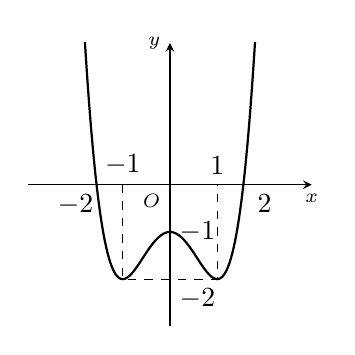
\begin{tikzpicture}[>=stealth,x=1cm,y=1cm,scale=0.6]
			\def\a{1} % Hệ số a phải khác 0
			\def\b{-2}
			\def\c{-1}
			\fill (-2,0) node[below]{$-2$};
			\fill (-1,0) node[above]{$-1$};
			\fill (1,0) node[above]{$1$};
			\fill (2,0) node[below]{$2$};
			\fill (0,-2) node[below right]{$-2$};
			\fill (0,-1) node[right]{$-1$};
			\draw[dashed] (-1,0)--(-1,-2)--(1,-2)--(1,0);
			\draw[->] (-3,0) -- (3,0) node[below] {\scriptsize $x$};
			\draw[->] (0,-3) -- (0,3) node[left] {\scriptsize $y$};
			\draw (0,0)node[below left]{\scriptsize $O$};
			\clip (-3,-3)rectangle(3,3);
			\draw[thick,samples=150,smooth,domain=-4:4] plot(\x,{\a*(\x)^4+(\b)*(\x)^2+(\c)});
	\end{tikzpicture}}
	\choice
	{$\left(-\infty-1\right)$}
	{$\left(-1;1\right)$}
	{\True $\left(-1;0\right)$}
	{$\left(0;1\right)$}
	\loigiai{
		Từ đồ thị, ta thấy hàm số đồng biến trên các khoảng $\left(-1;0\right)$ và $\left(1;+\infty\right)$.}
\end{ex}

\begin{ex}%[Phạm Hoàng Điệp]%[2D1Y1-2]%Câu 20
	[Mã 102 – 2020 – Lần 2] 
	\immini{Cho hàm số $y=f(x)$ có đồ thị là đường cong trong hình bên. Hàm số đã cho nghịch biến trên khoảng nào dưới đây?}{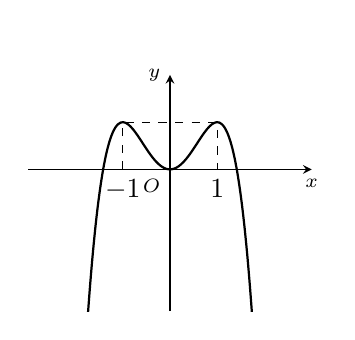
\begin{tikzpicture}[>=stealth,x=1cm,y=1cm,scale=0.6]
			\def\a{-1} % Hệ số a phải khác 0
			\def\b{2}
			\def\c{0}
			\fill (-1,0) node[below]{$-1$};
			\fill (1,0) node[below]{$1$};
			\draw[dashed] (-1,0)--(-1,1)--(1,1)--(1,0);
			\draw[->] (-3,0) -- (3,0) node[below] {\scriptsize $x$};
			\draw[->] (0,-3) -- (0,2) node[left] {\scriptsize $y$};
			\draw (0,0)node[below left]{\scriptsize $O$};
			\clip (-3,-3)rectangle(3,3);
			\draw[thick,samples=150,smooth,domain=-4:4] plot(\x,{\a*(\x)^4+(\b)*(\x)^2+(\c)});
	\end{tikzpicture}}
	\choice
	{\True $\left(-1;0\right)$}
	{$\left(-\infty ;-1\right)$}
	{$\left(0;1\right)$}
	{$\left(0;+\infty\right)$}
	\loigiai{
		Dựa vào đồ thị của hàm số $y=f(x)$ ta có hàm số $y=f(x)$ nghịch biến trên các khoảng $\left(-1;\,0\right)$ và $\left(1;\,+\infty\right)$, đồng biến trên các khoảng $\left(-\infty ;-1\right)$ và $\left(0;1\right).$}
\end{ex}

\begin{ex}%[Phạm Hoàng Điệp]%[2D1Y1-2]%Câu 21
	[Mã 107 – 2020 Lần 2] 
	\immini{Cho hàm số $y=f(x)$ có đồ thị là đường cong trong hình bên.}{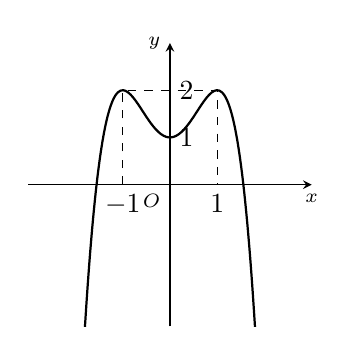
\begin{tikzpicture}[>=stealth,x=1cm,y=1cm,scale=0.6]
			\def\a{-1} % Hệ số a phải khác 0
			\def\b{2}
			\def\c{1}
			\fill (-1,0) node[below]{$-1$};
			\fill (0,1) node[right]{$1$};
			\fill (0,2) node[right]{$2$};
			\fill (1,0) node[below]{$1$};
			\draw[dashed] (-1,0)--(-1,2)--(1,2)--(1,0);
			\draw[->] (-3,0) -- (3,0) node[below] {\scriptsize $x$};
			\draw[->] (0,-3) -- (0,3) node[left] {\scriptsize $y$};
			\draw (0,0)node[below left]{\scriptsize $O$};
			\clip (-3,-3)rectangle(3,3);
			\draw[thick,samples=150,smooth,domain=-4:4] plot(\x,{\a*(\x)^4+(\b)*(\x)^2+(\c)});
	\end{tikzpicture}}
	Hàm số đã cho đồng biến trên khoảng nào dưới đây?
	\choice
	{\True $\left(0;1\right)$}
	{$\left(-\infty;0\right)$}
	{$\left(1;+\infty\right)$}
	{$\left(-1;0\right)$}
	\loigiai{
		Từ đồ thị hàm số $y=f(x)$ ta có hàm số đồng biến trên hai khoảng $\left(-\infty;-1\right)$ và $\left(0;1\right)$.}
\end{ex}

\begin{ex}%[Phạm Hoàng Điệp]%[2D1Y1-2]%Câu 22
	[Mã 103 – 2020 – Lần 2] 
	\immini{Cho hàm số $y=f(x)$ có đồ thị là đường cong hình bên. Hàm số đã cho đồng biến trên khoảng nào dưới đây?}{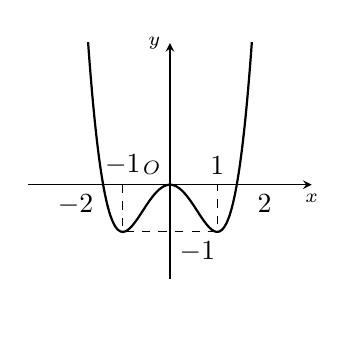
\begin{tikzpicture}[>=stealth,x=1cm,y=1cm,scale=0.6]
			\def\a{1} % Hệ số a phải khác 0
			\def\b{-2}
			\def\c{0}
			\fill (-2,0) node[below]{$-2$};
			\fill (-1,0) node[above]{$-1$};
			\fill (1,0) node[above]{$1$};
			\fill (2,0) node[below]{$2$};
			\fill (0,-1) node[below right]{$-1$};
			\draw[dashed] (-1,0)--(-1,-1)--(1,-1)--(1,0);
			\draw[->] (-3,0) -- (3,0) node[below] {\scriptsize $x$};
			\draw[->] (0,-2) -- (0,3) node[left] {\scriptsize $y$};
			\draw (0,0)node[above left]{\scriptsize $O$};
			\clip (-3,-3)rectangle(3,3);
			\draw[thick,samples=150,smooth,domain=-4:4] plot(\x,{\a*(\x)^4+(\b)*(\x)^2+(\c)});
	\end{tikzpicture}}
	\choice
	{\True $\left(-1;0\right)$}
	{$\left(-\infty ;-1\right)$}
	{$\left(0;+\infty\right)$}
	{$\left(0;1\right)$}
	\loigiai{
	}
\end{ex}

\begin{ex}%[Phạm Hoàng Điệp]%[2D1Y1-2]%Câu 23
	\immini{Cho hàm số $y=f(x)$ có đồ thị như hình vẽ bên. Hàm số đã cho đồng biến trên khoảng nào dưới đây?}{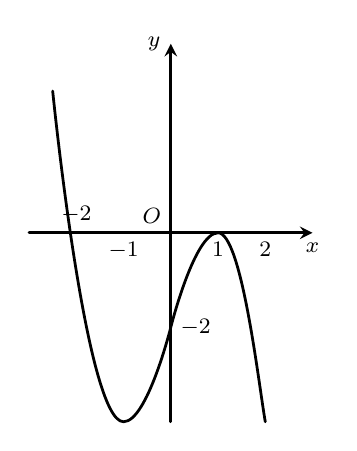
\begin{tikzpicture}[>=stealth,line join=round,line cap=round,font=\footnotesize,scale=.6]
			\def\xmin{-3} \def\xmax{3}
			\def\ymin{-4} \def\ymax{4} 
			\draw[->,line width=1pt] (\xmin,0)--(\xmax,0) node [below]{$x$};
			\draw[->,line width=1pt] (0,\ymin)--(0,\ymax) node [left]{$y$};
			\node at (0,0) [above left]{$O$};
			\fill (-2,0) node[above]{$-2$};
			\fill (-1,0) node[below]{$-1$};
			\fill (1,0) node[below]{$1$};
			\fill (2,0) node[below]{$2$};
			\fill (0,-2) node[right]{$-2$};
			\draw[line width=1pt]
			(-2.5,3)
			.. controls + (70:0) and + (180:0.8) .. (-1,-4)
			.. controls + (0:0.5) and + (-120:0) .. (0,-2)
			.. controls + (60:0) and + (180:0.5) .. (1,0)
			.. controls + (0:0.5) and + (100:0.8) .. (2,-4);
			(-3.5,-1)
			\draw[dashed]
			;
	\end{tikzpicture}}
	\choice
	{$\left(-\infty ;-1\right)$}
	{\True $\left(-1;1\right)$}
	{$\left(0;+\infty\right)$}
	{$\left(-\infty ;+\infty\right)$}
	\loigiai{
		Nhìn vào đồ thị đã cho, ta có hàm số đồng biến trên khoảng $\left(-1;1\right)$.}
\end{ex}

\begin{ex}%[Phạm Hoàng Điệp]%[2D1Y1-2]%Câu 24
	\immini{Cho hàm số $y=f(x)$ có đồ thị như hình vẽ bên. Hàm số đã cho nghịch biến trên khoảng nào dưới đây?}{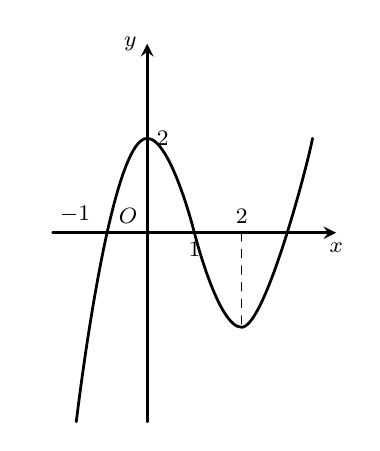
\begin{tikzpicture}[>=stealth,line join=round,line cap=round,font=\footnotesize,scale=.6]
			\def\xmin{-2} \def\xmax{4}
			\def\ymin{-4} \def\ymax{4} 
			\draw[->,line width=1pt] (\xmin,0)--(\xmax,0) node [below]{$x$};
			\draw[->,line width=1pt] (0,\ymin)--(0,\ymax) node [left]{$y$};
			\node at (0,0) [above left]{$O$};
			\fill (-1,0) node[above left]{$-1$};
			\fill (1,0) node[below]{$1$};
			\fill (2,0) node[above]{$2$};
			\fill (0,2) node[right]{$2$};
			\draw[line width=1pt]
			(-1.5,-4)
			.. controls + (70:0) and + (180:0.8) ..(0,2)
			.. controls + (0:0.5) and + (80:0) ..(1,0)
			.. controls + (100:0) and + (180:0.5) ..(2,-2)
			.. controls + (0:0.5) and + (-100:0.5) ..(3.5,2)
			(-2.5,3);
			\draw[dashed] (2,0)--(2,-2)
			;
	\end{tikzpicture}}
	\choice
	{$\left(-1;1\right)$}
	{$\left(-1;2\right)$}
	{\True $\left(1;2\right)$}
	{$\left(2;+\infty\right)$}
	\loigiai{
		Nhìn vào đồ thị đã cho, ta có hàm số nghịch biến trên khoảng $\left(0;2\right)$ nên nghịch biến trên khoảng $\left(1;2\right).$}
\end{ex}

\begin{ex}%[Phạm Hoàng Điệp]%[2D1Y1-2]%Câu 25
	\immini{Cho hàm số $y=f(x)$ có đồ thị như hình vẽ bên. Hàm số đã cho nghịch biến trên khoảng nào dưới đây?}{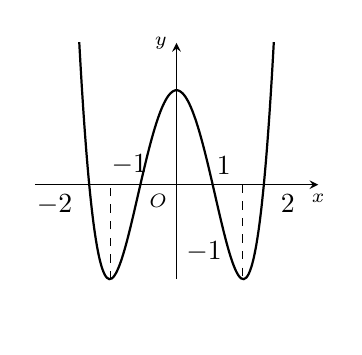
\begin{tikzpicture}[>=stealth,x=1cm,y=1cm,scale=0.6]
			\def\a{1} % Hệ số a phải khác 0
			\def\b{-4}
			\def\c{2}
			\fill (-2,0) node[below left]{$-2$};
			\fill (-1,0) node[above]{$-1$};
			\fill (1,0) node[above]{$1$};
			\fill (2,0) node[below right]{$2$};
			\fill (0,-1) node[below right]{$-1$};
			\draw[dashed] (-1.4,-2)--(-1.4,0) (1.4,0)--(1.4,-2);
			\draw[->] (-3,0) -- (3,0) node[below] {\scriptsize $x$};
			\draw[->] (0,-2) -- (0,3) node[left] {\scriptsize $y$};
			\draw (0,0)node[below left]{\scriptsize $O$};
			\clip (-3,-3)rectangle(3,3);
			\draw[thick,samples=150,smooth,domain=-4:4] plot(\x,{\a*(\x)^4+(\b)*(\x)^2+(\c)});
	\end{tikzpicture}}
	\choice
	{$\left(-\infty ;-1\right)$}
	{$\left(-1;1\right)$}
	{$\left(1;2\right)$}
	{\True $\left(0;1\right)$}
	\loigiai{
		Nhìn vào đồ thị đã cho, ta có trên khoảng $\left(0;1\right)$ đồ thị hàm số đi xuống (theo chiều từ trái qua phải) nên nghịch biến trên khoảng $\left(0;1\right).$}
\end{ex}

\begin{ex}%[Phạm Hoàng Điệp]%[2D1Y1-2]%Câu 26
	\immini{Cho hàm số $y=f(x)$ có đồ thị như hình vẽ bên.}{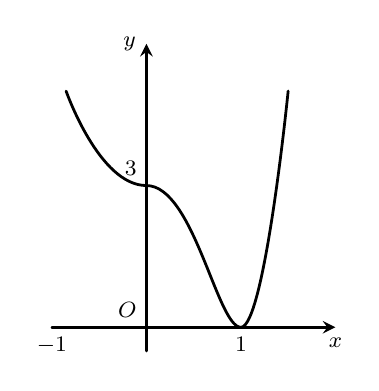
\begin{tikzpicture}[>=stealth,line join=round,line cap=round,font=\footnotesize,scale=.6]
			\def\xmin{-2} \def\xmax{4}
			\def\ymin{-0.5} \def\ymax{6} 
			\draw[->,line width=1pt] (\xmin,0)--(\xmax,0) node [below]{$x$};
			\draw[->,line width=1pt] (0,\ymin)--(0,\ymax) node [left]{$y$};
			\node at (0,0) [above left]{$O$};
			\fill (-2,0) node[below]{$-1$};
			\fill (2,0) node[below]{$1$};
			\fill (0,3) node[above left]{$3$};
			\draw[line width=1pt]
			(-1.7,5)
			.. controls + (70:0) and + (180:1) ..(0,3)
			.. controls + (0:1) and + (180:0.5) ..(2,0)
			.. controls + (0:0.5) and + (120:0) ..(3,5);
			\draw[dashed]
			;
	\end{tikzpicture}}
	Mệnh đề nào sau đây là đúng?
	\choice
	{Hàm số đã cho đồng biến trên khoảng $\left(0;2\right)$}
	{Hàm số đã cho đồng biến trên khoảng $\left(-1;+\infty\right)$}
	{Hàm số đã cho nghịch biến trên khoảng $\left(-1;2\right)$}
	{\True Hàm số đã cho nghịch biến trên khoảng $\left(-\infty ;1\right)$}
	\loigiai{
		Nhìn vào đồ thị đã cho, ta có trên khoảng $\left(-\infty ;1\right)$ đồ thị hàm số đi xuống (theo chiều từ trái qua phải) nên nghịch biến trên khoảng $\left(-\infty ;1\right)$.}
\end{ex}

\begin{ex}%[Phạm Hoàng Điệp]%[2D1Y1-2]%Câu 27
	\immini{Cho hàm số $y=f(x)$ có đồ thị như hình vẽ. Hàm số đã cho đồng biến trên khoảng nào?}{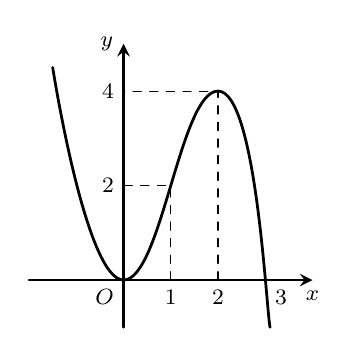
\begin{tikzpicture}[>=stealth,line join=round,line cap=round,font=\footnotesize,scale=.6]
			\def\xmin{-2} \def\xmax{4}
			\def\ymin{-1} \def\ymax{5} 
			\draw[->,line width=1pt] (\xmin,0)--(\xmax,0) node [below]{$x$};
			\draw[->,line width=1pt] (0,\ymin)--(0,\ymax) node [left]{$y$};
			\node at (0,0) [below left]{$O$};
			\fill (1,0) node[below]{$1$};
			\fill (2,0) node[below]{$2$};
			\fill (3,0) node[below right]{$3$};
			\fill (0,2) node[left]{$2$};
			\fill (0,4) node[left]{$4$};
			\draw[line width=1pt]
			(-1.5,4.5)
			.. controls + (70:0) and + (180:0.8) ..(0,0)
			.. controls + (0:0.8) and + (180:0.8) ..(2,4)
			.. controls + (0:0.8) and + (100:0.5) ..(3.1,-1);
			\draw[dashed] (1,0)--(1,2)--(0,2) (2,0)--(2,4)--(0,4);
	\end{tikzpicture}}
	
	\choice
	{$\left(-\infty;0\right)$}
	{$\left(1;3\right)$}
	{\True $\left(0;2\right)$}
	{$\left(0;+\infty\right)$}
	\loigiai{}
\end{ex}

\begin{ex}%[Phạm Hoàng Điệp]%[2D1Y1-2]%Câu 28
	\immini{Cho hàm số $y=f(x)$ có đồ thị như hình vẽ. Hàm số đã cho nghịch biến trên khoảng nào?}{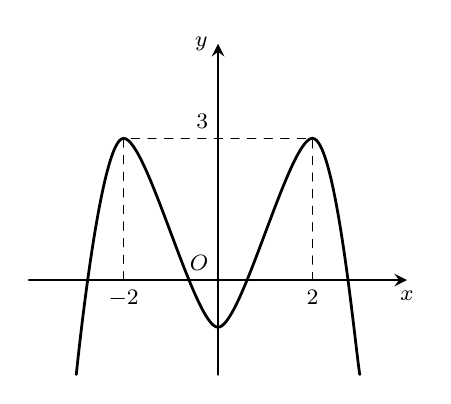
\begin{tikzpicture}[>=stealth,line join=round,line cap=round,font=\footnotesize,scale=.6]
			\def\xmin{-4} \def\xmax{4}
			\def\ymin{-2} \def\ymax{5} 
			\draw[->,line width=1pt] (\xmin,0)--(\xmax,0) node [below]{$x$};
			\draw[->,line width=1pt] (0,\ymin)--(0,\ymax) node [left]{$y$};
			\node at (0,0) [above left]{$O$};
			\fill (-2,0) node[below]{$-2$};
			\fill (2,0) node[below]{$2$};
			\fill (0,3) node[above left]{$3$};
			\draw[line width=1pt]
			(-3,-2)
			.. controls + (70:0) and + (180:0.5) ..(-2,3)
			.. controls + (0:0.5) and + (180:0.5) ..(0,-1)
			.. controls + (0:0.5) and + (180:0.5) ..(2,3)
			.. controls + (0:0.5) and + (100:0.5) ..(3,-2);
			\draw[dashed] (-2,0)--(-2,3)--(2,3)--(2,0);
	\end{tikzpicture}}
	\choice
	{\True $\left(-2;0\right)$}
	{$\left(-\infty;0\right)$}
	{$\left(-2;2\right)$}
	{$\left(0;2\right)$}
	\loigiai{}
\end{ex}

\begin{ex}%[Phạm Hoàng Điệp]%[2D1Y1-2]%Câu 29
	\immini{Cho hàm số $y=f(x)$ có đồ thị như hình vẽ. Hàm số đã cho nghịch biến trên khoảng nào?}{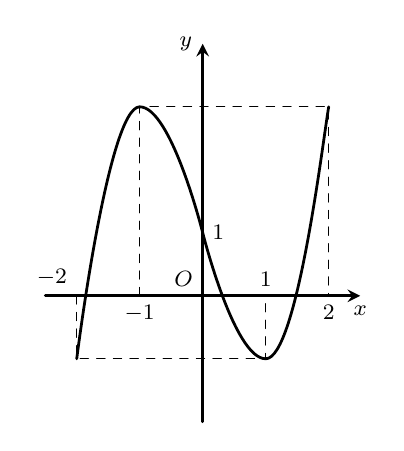
\begin{tikzpicture}[>=stealth,line join=round,line cap=round,font=\footnotesize,scale=.8]
			\def\xmin{-2.5} \def\xmax{2.5}
			\def\ymin{-2} \def\ymax{4} 
			\draw[->,line width=1pt] (\xmin,0)--(\xmax,0) node [below]{$x$};
			\draw[->,line width=1pt] (0,\ymin)--(0,\ymax) node [left]{$y$};
			\node at (0,0) [above left]{$O$};
			\fill (-2,0) node[above left]{$-2$};
			\fill (-1,0) node[below]{$-1$};
			\fill (1,0) node[above]{$1$};
			\fill (2,0) node[below]{$2$};
			\fill (0,1) node[right]{$1$};
			\draw[line width=1pt]
			(-2,-1)
			.. controls + (70:0) and + (180:0.5) ..(-1,3)
			.. controls + (0:0.5) and + (120:0) ..(0,1)
			.. controls + (60:0) and + (180:0.5) ..(1,-1)
			.. controls + (0:0.5) and + (-100:0.5) ..(2,3);
			\draw[dashed] (-2,0)--(-2,-1)--(1,-1)--(1,0) (-1,0)--(-1,3)--(2,3)--(2,0);
	\end{tikzpicture}}
	
	\choice
	{\True $\left(-1;1\right)$}
	{$\left(-2;-1\right)$}
	{$\left(-1;2\right)$}
	{$\left(1;+\infty\right)$}
	\loigiai{}
\end{ex}

\begin{ex}%[Phạm Hoàng Điệp]%[2D1Y1-2]%Câu 30
	[Chuyên ĐH Vinh-Nghệ An-2020] 
	\immini{Cho hàm số $y=f(x)$ có đồ thị như hình vẽ bên.}{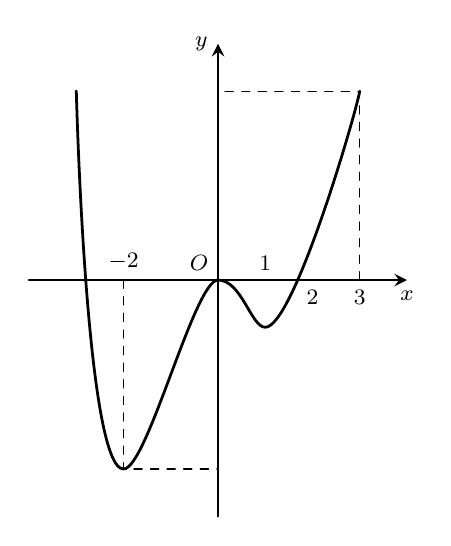
\begin{tikzpicture}[>=stealth,line join=round,line cap=round,font=\footnotesize,scale=.6]
			\def\xmin{-4} \def\xmax{4}
			\def\ymin{-5} \def\ymax{5} 
			\draw[->,line width=1pt] (\xmin,0)--(\xmax,0) node [below]{$x$};
			\draw[->,line width=1pt] (0,\ymin)--(0,\ymax) node [left]{$y$};
			\node at (0,0) [above left]{$O$};
			\fill (-2,0) node[above]{$-2$};
			\fill (1,0) node[above]{$1$};
			\fill (2,0) node[below]{$2$};
			\fill (3,0) node[below]{$3$};
			\draw[line width=1pt]
			(-3,4)
			.. controls + (70:0) and + (180:0.8) ..(-2,-4)
			.. controls + (0:0.5) and + (180:0.5) ..(0,0)
			.. controls + (0:0.5) and + (180:0.3) ..(1,-1)
			.. controls + (0:0.6) and + (-100:0.5) ..(3,4)
			;
			\draw[dashed] (-2,0)--(-2,-4)--(0,-4) (3,0)--(3,4)--(0,4);
	\end{tikzpicture}}
	Hàm số đã cho nghịch biến trên khoảng
	\choice
	{$\left(-1;0\right)$}
	{$\left(-2;-1\right)$}
	{\True $\left(0;1\right)$}
	{$\left(1;3\right)$}
	\loigiai
	{Từ đồ thị hàm số ta có hàm số nghịch biến trên các khoảng $\left(-\infty;-2\right)$ và $\left(0;1\right)$.}
\end{ex}

\begin{ex}%[Phạm Hoàng Điệp]%[2D1Y1-2]%Câu 31
	[Chuyên Hưng Yên-2020] 
	\immini{Cho hàm số $f(x)$ liên tục trên $\mathbb{R}$ và có đồ thị như hình vẽ bên. Khẳng định nào sau đây là đúng?}{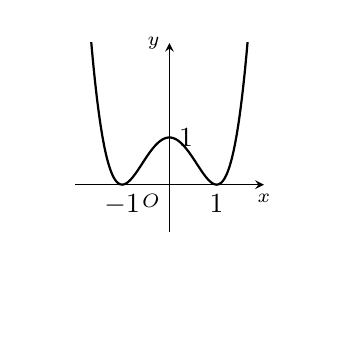
\begin{tikzpicture}[>=stealth,x=1cm,y=1cm,scale=0.6]
			\def\a{1} % Hệ số a phải khác 0
			\def\b{-2}
			\def\c{1}
			\fill (-1,0) node[below]{$-1$};
			\fill (0,1) node[right]{$1$};
			\fill (1,0) node[below]{$1$};
			\draw[->] (-2,0) -- (2,0) node[below] {\scriptsize $x$};
			\draw[->] (0,-1) -- (0,3) node[left] {\scriptsize $y$};
			\draw (0,0)node[below left]{\scriptsize $O$};
			\clip (-3,-3)rectangle(3,3);
			\draw[thick,samples=150,smooth,domain=-4:4] plot(\x,{\a*(\x)^4+(\b)*(\x)^2+(\c)});
	\end{tikzpicture}}
	\choice
	{Hàm số đồng biến trên$\left(-\infty;0\right)$ và$\left(0;+\infty\right)$}
	{\True Hàm số đồng biến trên$\left(-1;0\right)$ và$\left(1;+\infty\right)$}
	{Hàm số đồng biến trên$\left(-1;0\right)\cup\left(1;+\infty\right)$}
	{Hàm số đồng biến trên$\left(-\infty ;-1\right)\cup\left(1;+\infty\right)$}
	\loigiai
	{Hàm số đồng biến trên$\left(-1;0\right)$ và$\left(1;+\infty\right)$.
	}
\end{ex}

\begin{ex}%[Phạm Hoàng Điệp]%[2D1Y1-2]%Câu 32
	[Mã 101-2021 Lần 1]
	\immini{ Cho hàm số $y=f(x)$ có đồ thị là đường cong trong hình bên.}{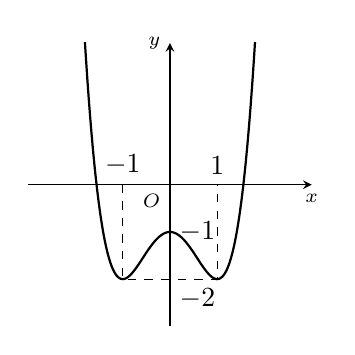
\begin{tikzpicture}[>=stealth,x=1cm,y=1cm,scale=0.6]
			\def\a{1} % Hệ số a phải khác 0
			\def\b{-2}
			\def\c{-1}
			\fill (-1,0) node[above]{$-1$};
			\fill (1,0) node[above]{$1$};
			\fill (0,-2) node[below right]{$-2$};
			\fill (0,-1) node[right]{$-1$};
			\draw[dashed] (-1,0)--(-1,-2)--(1,-2)--(1,0);
			\draw[->] (-3,0) -- (3,0) node[below] {\scriptsize $x$};
			\draw[->] (0,-3) -- (0,3) node[left] {\scriptsize $y$};
			\draw (0,0)node[below left]{\scriptsize $O$};
			\clip (-3,-3)rectangle(3,3);
			\draw[thick,samples=150,smooth,domain=-4:4] plot(\x,{\a*(\x)^4+(\b)*(\x)^2+(\c)});
	\end{tikzpicture}}
	Hàm số đã cho nghịch biến trong khoảng nào dưới đây?
	\choice
	{\True $\left(0;1\right)$}
	{$\left(-\infty ;0\right)$}
	{$\left(0;+\infty\right)$}
	{$\left(-1;1\right)$}
	\loigiai{
		Ta có hàm số nghịch biến trên khoảng $\left(0;1\right)$.}
\end{ex}

\begin{ex}%[Phạm Hoàng Điệp]%[2D1Y1-2]%Câu 33
	[Mã 103-2021-Lần 1] 
	\immini{Cho hàm số $y=f(x)$ có đồ thị là đường cong trong hình bên. Hàm số đã cho đồng biến trên khoảng nào dưới đây?}{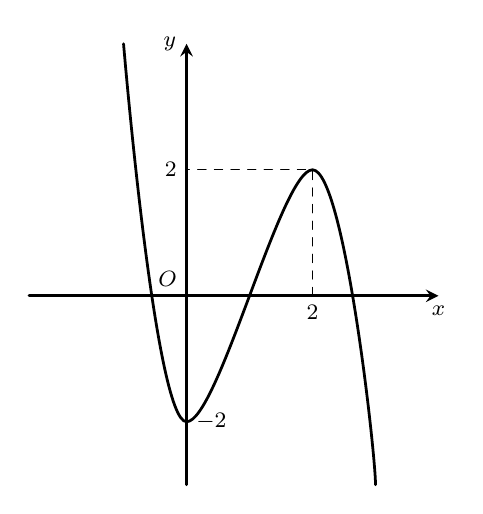
\begin{tikzpicture}[>=stealth,line join=round,line cap=round,font=\footnotesize,scale=.8]
			\def\xmin{-2.5} \def\xmax{4}
			\def\ymin{-3} \def\ymax{4} 
			\draw[->,line width=1pt] (\xmin,0)--(\xmax,0) node [below]{$x$};
			\draw[->,line width=1pt] (0,\ymin)--(0,\ymax) node [left]{$y$};
			\node at (0,0) [above left]{$O$};
			\fill (2,0) node[below]{$2$};
			\fill (0,2) node[left]{$2$};
			\fill (0,-2) node[right]{$-2$};
			\draw[line width=1pt]
			(-1,4)
			.. controls + (70:0) and + (180:0.5) ..(0,-2)
			.. controls + (0:0.5) and + (180:0.5) ..(2,2)
			.. controls + (0:0.5) and + (90:0.5) ..(3,-3)
			;
			\draw[dashed] (2,0)--(2,2)--(0,2);
	\end{tikzpicture}}
	\choice
	{$\left(-\infty ;2\right)$}
	{\True $\left(0;2\right)$}
	{$\left(-2;2\right)$}
	{$\left(2;+\infty\right)$}
	\loigiai{
		Dựa vào đồ thị hàm số ta có hàm số đồng biến trên khoảng $\left(0;2\right)$.}
\end{ex}

\begin{ex}%[Phạm Hoàng Điệp]%[2D1Y1-2]%Câu 34
	[Mã 102-2021 Lần 1]
	\immini{Cho hàm số $y=f(x)$ có đồ thị là đường cong trong hình bên. Hàm số đã cho đồng biến trên khoảng nào dưới đây?}{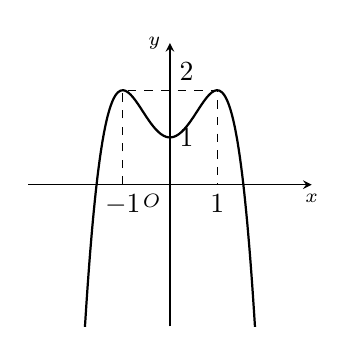
\begin{tikzpicture}[>=stealth,x=1cm,y=1cm,scale=0.6]
			\def\a{-1} % Hệ số a phải khác 0
			\def\b{2}
			\def\c{1}
			\fill (-1,0) node[below]{$-1$};
			\fill (0,1) node[right]{$1$};
			\fill (0,2) node[above right]{$2$};
			\fill (1,0) node[below]{$1$};
			\draw[dashed] (-1,0)--(-1,2)--(1,2)--(1,0);
			\draw[->] (-3,0) -- (3,0) node[below] {\scriptsize $x$};
			\draw[->] (0,-3) -- (0,3) node[left] {\scriptsize $y$};
			\draw (0,0)node[below left]{\scriptsize $O$};
			\clip (-3,-3)rectangle(3,3);
			\draw[thick,samples=150,smooth,domain=-4:4] plot(\x,{\a*(\x)^4+(\b)*(\x)^2+(\c)});
	\end{tikzpicture}}
	\choice
	{$\left(-1;1\right)$}
	{$\left(-\infty;0\right)$}
	{\True $\left(0;1\right)$}
	{$\left(0;+\infty\right)$}
	\loigiai{
		Nhìn đồ thị ta thấy hàm số đã cho đồng biến trên $\left(0;1\right)$.}
\end{ex}

\begin{ex}%[Phạm Hoàng Điệp]%[2D1Y1-2]%Câu 35
	[Mã 104-2021 Lần 1] 
	\immini{Cho hàm số $y=f(x)$ có đồ thị là đường cong trong hình bên.}{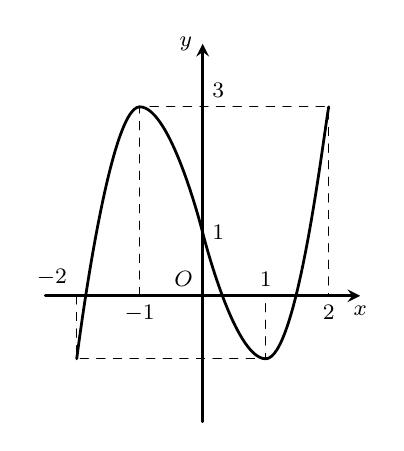
\begin{tikzpicture}[>=stealth,line join=round,line cap=round,font=\footnotesize,scale=.8]
			\def\xmin{-2.5} \def\xmax{2.5}
			\def\ymin{-2} \def\ymax{4} 
			\draw[->,line width=1pt] (\xmin,0)--(\xmax,0) node [below]{$x$};
			\draw[->,line width=1pt] (0,\ymin)--(0,\ymax) node [left]{$y$};
			\node at (0,0) [above left]{$O$};
			\fill (-2,0) node[above left]{$-2$};
			\fill (-1,0) node[below]{$-1$};
			\fill (1,0) node[above]{$1$};
			\fill (2,0) node[below]{$2$};
			\fill (0,1) node[right]{$1$};
			\fill (0,3) node[above right]{$3$};
			\draw[line width=1pt]
			(-2,-1)
			.. controls + (70:0) and + (180:0.5) ..(-1,3)
			.. controls + (0:0.5) and + (120:0) ..(0,1)
			.. controls + (60:0) and + (180:0.5) ..(1,-1)
			.. controls + (0:0.5) and + (-100:0.5) ..(2,3);
			\draw[dashed] (-2,0)--(-2,-1)--(1,-1)--(1,0) (-1,0)--(-1,3)--(2,3)--(2,0);
	\end{tikzpicture}}
	Hàm số đã cho nghịch biến trên khoảng nào dưới đây?
	\choice
	{\True $\left(-1;1\right)$}
	{$\left(1;+\infty\right)$}
	{$\left(-\infty ;1\right)$}
	{$\left(0;3\right)$}
	\loigiai{
		Từ hình vẽ ta thấy hàm số đã cho nghịch biến trên khoảng $\left(-1;\,1\right)$.}
\end{ex}

\begin{ex}%[Phạm Hoàng Điệp]%[2D1Y1-2]%Câu 36
	[Đề Minh Họa 2021] Cho hàm số $f(x)$ có bảng biến thiên như sau:
	\begin{center}
		\begin{tikzpicture}[>=stealth]
			\tkzTabInit[nocadre,lgt=1.2,espcl=2,deltacl=0.5]{$x$/.7 ,$f'(x)$/.7,$f(x)$/2}
			{$-\infty$ , $-2$ , $0$ , $2$ , $+\infty$}
			\tkzTabLine{ , + , $0$ , - , $0$ , + , $0$ , - , }
			\tkzTabVar{-/$-\infty$ , +/$1$, -/$-1$ , +/$1$ , -/$-\infty$}
		\end{tikzpicture}	
	\end{center}
	Hàm số đã cho đồng biến trên khoảng nào, trong các khoảng dưới đây?
	\choice
	{$\left(-2;2\right)$}
	{\True $\left(0;2\right)$}
	{$\left(-2;0\right)$}
	{$\left(2;+\infty\right)$}
	\loigiai{
		Từ bảng biến thiên ta thấy hàm số đồng biến trên khoảng $\left(0;2\right)$.}
\end{ex}

\begin{ex}%[Phạm Hoàng Điệp]%[2D1Y1-2]%Câu 37
	[Đề minh họa 2022] Cho hàm số $y=f(x)$ có bảng biến thiên như sau:
	\begin{center}
		\begin{tikzpicture}[>=stealth]
			\tkzTabInit[nocadre,lgt=1.2,espcl=2,deltacl=0.5]{$x$/.7 ,$f'(x)$/.7,$f(x)$/2}
			{$-\infty$ , $-2$ , $0$ , $2$ , $+\infty$}
			\tkzTabLine{ , - , $0$ , + , $0$ , - , $0$ , + , }
			\tkzTabVar{+/$+\infty$ , -/$-1$, +/$1$ , -/$-1$ , +/$+\infty$}
		\end{tikzpicture}
	\end{center}
	Hàm số đã cho đồng biến trên khoảng nào dứoi đây?
	\choice
	{$\left(0;+\infty\right)$}
	{$\left(-\infty ;-2\right)$}
	{$\left(0;2\right)$}
	{\True $\left(-2;0\right)$}
	\loigiai{
		Dựa vào bảng biến thiên ta thấy đồ thị hàm số đồng biến trên $\left(-2;0\right)$ và $\left(2;+\infty\right)$.}
\end{ex}

\begin{ex}%[Phạm Hoàng Điệp]%[2D1Y1-2]%Câu 38
	[Mã 101-2022] Cho hàm số $y=f(x)$ có bảng biến thiên như sau:
	\begin{center}
		\begin{tikzpicture}[>=stealth]
			\tkzTabInit[nocadre,lgt=1.2,espcl=2,deltacl=0.5]{$x$/.7 ,$f'(x)$/.7,$f(x)$/2}
			{$-\infty$ , $-1$ , $0$ , $1$ , $+\infty$}
			\tkzTabLine{ , - , $0$ , + , $0$ , - , $0$ , + , }
			\tkzTabVar{+/$+\infty$ , -/$0$, +/$3$ , -/$0$ , +/$+\infty$}
		\end{tikzpicture}
	\end{center}
	Hàm số đã cho nghịch biến trên khoảng nào dưới đây?
	\choice
	{$\left(1+\infty\right)$}
	{\True $\left(0;1\right)$}
	{$\left(-1;0\right)$}
	{$\left(0;+\infty\right)$}
	\loigiai{
		Chọn B}
\end{ex}

\begin{ex}%[Phạm Hoàng Điệp]%[2D1Y1-2]%Câu 39
	[Mã 102-2022] Cho hàm số $y=f(x)$ có bảng biến thiên như sau:
	\begin{center}
		\begin{tikzpicture}[>=stealth]
			\tkzTabInit[nocadre,lgt=1.2,espcl=2,deltacl=0.5]{$x$/.7 ,$f'(x)$/.7,$f(x)$/2}
			{$-\infty$ , $-1$ , $0$ , $1$ , $+\infty$}
			\tkzTabLine{ , - , $0$ , + , $0$ , - , $0$ , + , }
			\tkzTabVar{+/$+\infty$ , -/$0$, +/$3$ , -/$0$ , +/$+\infty$}
		\end{tikzpicture}
	\end{center}
	Hàm số đã cho nghịch biến trên khoảng nào dưới đây?
	\choice
	{$\left(0;+\infty\right)$}
	{$\left(1;+\infty\right)$}
	{$\left(-1;0\right)$}
	{\True $\left(0;1\right)$}
	\loigiai{
		
	}
\end{ex}

\begin{ex}%[Phạm Hoàng Điệp]%[2D1Y1-2]%Câu 40
	[Mã 103-2022] Cho hàm số $y=f(x)$ có bảng biến thiên như sau:
	\begin{center}
		\begin{tikzpicture}[>=stealth]
			\tkzTabInit[nocadre,lgt=1.2,espcl=2,deltacl=0.5]{$x$/.7 ,$f'(x)$/.7,$f(x)$/2}
			{$-\infty$ , $-1$ , $0$ , $1$ , $+\infty$}
			\tkzTabLine{ , - , $0$ , + , $0$ , - , $0$ , + , }
			\tkzTabVar{+/$+\infty$ , -/$0$, +/$3$ , -/$0$ , +/$+\infty$}
		\end{tikzpicture}
	\end{center}
	Hàm số đã cho đồng biến trên khoảng nào dưới đây?
	\choice
	{$\left(0;3\right)$}
	{$\left(0;+\infty\right)$}
	{\True $\left(-1;0\right)$}
	{$\left(-\infty ;-1\right)$}
	\loigiai{
		Chọn C}
\end{ex}

\begin{ex}%[Phạm Hoàng Điệp]%[2D1Y1-2]%Câu 41
	[Mã 104-2022] Cho hàm số $y=f(x)$ có bảng biến thiên như sau:
	\begin{center}
		\begin{tikzpicture}[>=stealth]
			\tkzTabInit[nocadre,lgt=1.2,espcl=2,deltacl=0.5]{$x$/.7 ,$f'(x)$/.7,$f(x)$/2}
			{$-\infty$ , $-1$ , $0$ , $1$ , $+\infty$}
			\tkzTabLine{ , - , $0$ , + , $0$ , - , $0$ , + , }
			\tkzTabVar{+/$+\infty$ , -/$0$, +/$3$ , -/$0$ , +/$+\infty$}
		\end{tikzpicture}
	\end{center}
	Hàm số đã cho đồng biến trên khoảng nào dưới đây?
	\choice
	{$\left(-\infty;-1\right)$}
	{$\left(0;3\right)$}
	{$\left(0;+\infty\right)$}
	{\True $\left(-1;0\right)$}
	\loigiai{
		Ta có đồ thị tăng trên khoảng $\left(-1;0\right)$, nên đó là đáp án đúng.}
\end{ex}
\begin{dang}{Tìm khoảng đơn điệu của hàm số cho trước}
\end{dang}
\begin{ex}%[2D1Y1-1]
	[Mã 110-2017]
	Hàm số nào dưới đây đồng biến trên khoảng $\left(-\infty ;+\infty\right)$?
	\choice
	{$ y=\dfrac{x-1}{x-2}$}
	{\True $ y=x^3+x$}
	{$ y=-x^3-3x$}
	{$ y=\dfrac{x+1}{x+3}$}
	\loigiai{
		Vì $ y=x^3+x\Rightarrow{y}'=3x^2+1>0$, $\forall x\in\mathbb{R}$.
	}
\end{ex}
\begin{ex}%[2D1Y1-1]
	[Đề Tham Khảo - 2017]
	Cho hàm số $y=\dfrac{x-2}{x+1}$. Mệnh đề nào dưới đây đúng?
	\choice
	{Hàm số nghịch biến trên khoảng $\left(-\infty ;+\infty\right)$}
	{Hàm số nghịch biến trên khoảng $\left(-1;+\infty\right)$}
	{Hàm số nghịch biến trên khoảng $\left(-\infty ;-1\right)$}
	{\True Hàm số đồng biến trên khoảng $\left(-\infty ;-1\right)$}
	\loigiai{
		Tập xác định $\mathscr{D}=\mathbb{R}\backslash\left\{-1\right\}$.\\
		Ta có $y'=\dfrac{3}{\left(x+1\right)^2}>0$, $\forall x\in\mathbb{R}\backslash\left\{-1\right\}$.
	}
\end{ex}
\begin{ex}%[2D1Y1-1]
	[Đề Tham Khảo - 2017]
	Hàm số nào dưới đây đồng biến trên khoảng $\left(-\infty ;+\infty\right)$?
	\choice
	{$ y=x^4+3x^2$}
	{$ y=\dfrac{x-2}{x+1}$}
	{\True $ y=3x^3+3x-2$}
	{$ y=2x^3-5x+1$}
	\loigiai{
		Hàm số $ y=3x^3+3x-2$ có tập xác định là $\mathscr{D}=\mathbb{R}$.\\
		$y'=9x^2+3>0,\forall x\in\mathbb{R}$, suy ra hàm số đồng biến trên khoảng $\left(-\infty ;+\infty\right)$.
	}
\end{ex}
\begin{ex}%[2D1Y1-1]
	[Mã 110 - 2017]
	Cho hàm số $ y=x^3-3x^2$. Mệnh đề nào dưới đây đúng?
	\choice
	{Hàm số đồng biến trên khoảng $\left(0;2\right)$}
	{\True Hàm số nghịch biến trên khoảng $\left(0;2\right)$}
	{Hàm số nghịch biến trên khoảng $\left(-\infty ;0\right)$}
	{Hàm số nghịch biến trên khoảng $\left(2;+\infty\right)$}
	\loigiai{
		Ta có $y'=3x^2-6x$; $y'=0\Leftrightarrow\left[\begin{aligned}
			&x=0\\ 
			&x=2\\ 
		\end{aligned}\right.$.\\
		Lập bảng biến thiên rồi suy ra hàm số nghịch biến trên khoảng $\left(0;2\right)$.
	}
\end{ex}
\begin{ex}%[2D1Y1-1]
	[Đề Minh Họa - 2017]
	Hỏi hàm số $y=2x^4+1$ đồng biến trên khoảng nào?
	\choice
	{$\left(-\infty ;0\right)$}
	{$\left(-\infty ;-\dfrac{1}{2}\right)$}
	{\True $\left(0;+\infty\right)$}
	{$\left(-\dfrac{1}{2};+\infty\right)$}
	\loigiai{
		Tập xác định $\mathscr{D}=\mathbb{R}$\\
		Ta có $y'=8x^3$; $ y'=0\Leftrightarrow 8x^3=0\Leftrightarrow x=0$ suy ra $ y(0)=1$\\
		Giới hạn: $\underset{x\to-\infty}{\lim}\,y=+\infty$; $\underset{x\to+\infty}{\lim}\,y=+\infty$\\
		Bảng biến thiên
		\begin{center}
			\begin{tikzpicture}
				\tkzTabInit[nocadre,lgt=1.2,espcl=3]{$x$/0.8,$f'(x)$/0.8,$f(x)$/2}{$-\infty$,$0$,$+\infty$}
				\tkzTabLine{,-,0,+,}
				\tkzTabVar{+/$+\infty$,-/$1$,+/$+\infty$}
			\end{tikzpicture}
		\end{center}
		Vậy hàm số đồng biến trên khoảng $\left(0;+\infty\right)$.
	}
\end{ex}
\begin{ex}%[2D1Y1-1]
	[Mã 105 - 2017]%Câu 6
	Cho hàm số $y=f(x)$ có đạo hàm $f'(x)=x^2+1$, $\forall x\in\mathbb{R}$. Mệnh đề nào dưới đây đúng?
	\choice
	{Hàm số nghịch biến trên khoảng $\left(1;+\infty\right)$}
	{Hàm số nghịch biến trên khoảng $\left(-1;1\right)$}
	{\True Hàm số đồng biến trên khoảng $\left(-\infty ;+\infty\right)$}
	{Hàm số nghịch biến trên khoảng $\left(-\infty ;0\right)$}
	\loigiai{
		Do hàm số $y=f(x)$ có đạo hàm $f'(x)=x^2+1>0$ $\forall x\in\mathbb{R}$ nên hàm số đồng biến trên khoảng $\left(-\infty ;+\infty\right)$.
	}
\end{ex}
\begin{ex}%[2D1Y1-1]
	[Mã 105 - 2017]%Câu 7
	Cho hàm số $ y=x^3-2x^2+x+1$. Mệnh đề nào dưới đây đúng?
	\choice
	{Hàm số nghịch biến trên khoảng $\left(1;+\infty\right)$}
	{\True Hàm số nghịch biến trên khoảng $\left(\dfrac{1}{3};1\right)$}
	{Hàm số nghịch biến trên khoảng $\left(-\infty ;\dfrac{1}{3}\right)$}
	{Hàm số đồng biến trên khoảng $\left(\dfrac{1}{3};1\right)$}
	\loigiai{
		Ta có $y'=3x^2-4x+1\Rightarrow{y}'=0\Leftrightarrow\left[\begin{aligned}
			&x=1\\ 
			&x=\dfrac{1}{3}\\ 
		\end{aligned}\right.$.\\
		Bảng biến thiên\\
		\begin{center}
			\begin{tikzpicture}
				\tkzTabInit[nocadre,lgt=1.2,espcl=3]{$x$/1.0,$f'(x)$/0.8,$f(x)$/2.5}{$-\infty$,$\dfrac{1}{3}$,$1$,$+\infty$}
				\tkzTabLine{,+,0,-,0,+,}
				\tkzTabVar{-/$-\infty$,+/$\dfrac{31}{27}$,-/$1$,+/$+\infty$}
			\end{tikzpicture}
		\end{center}
		Vậy hàm số nghịch biến trên khoảng $\left(\dfrac{1}{3};1\right)$.
	}
\end{ex}
\begin{ex}%[2D1Y1-1]
	[Mã 105 - 2017]%Câu 8
	Cho hàm số $ y=x^4-2x^2$. Mệnh đề nào dưới đây đúng?
	\choice
	{\True Hàm số nghịch biến trên khoảng $\left(-\infty ;-2\right)$}
	{Hàm số đồng biến trên khoảng $\left(-1;1\right)$}
	{Hàm số nghịch biến trên khoảng $\left(-1;1\right)$}
	{Hàm số đồng biến trên khoảng $\left(-\infty ;-2\right)$}
	\loigiai{
		Tập xác định $\mathscr{D}=\mathbb{R}.$\\
		$y'=4x^3-4x;y'=0\Leftrightarrow 4x^3-4x=0\Leftrightarrow\left[\begin{aligned}
			&x=0\\ 
			&x=1\\ 
			&x=-1\\ 
		\end{aligned}\right.$
		\begin{center}
			\begin{tikzpicture}
				\tkzTabInit[nocadre,lgt=1.2,espcl=2]{$x$/1,$f'(x)$/1,$f(x)$/2.5}{$-\infty$,$-1$,$0$,$1$,$+\infty$}
				\tkzTabLine{,-,0,+,0,-,0,+,}
				\tkzTabVar{+/$+\infty$,-/$1$,+/$0$,-/$-1$,+/$+\infty$}
			\end{tikzpicture}
		\end{center}
		Suy ra hàm số đồng biến trên các khoảng $\left(-1;0\right)$, $\left(1;+\infty\right)$; hàm số nghịch biến trên các khoảng $\left(-\infty ;-1\right)$, $\left(0;1\right)$.\\ Vậy hàm số nghịch biến trên khoảng $\left(-\infty ;-2\right)$.
	}
\end{ex}
\begin{ex}%[2D1Y1-1]
	[Mã 123 - 2017]%Câu 9
	Hàm số $ y=\dfrac{2}{x^2+1}$ nghịch biến trên khoảng nào dưới đây?
	\choice
	{$ (-\infty ;+\infty)$}
	{\True $ (0;+\infty)$}
	{$ (-\infty ;0)$}
	{$ (-1;1)$}
	\loigiai{
		Ta có $y'=\dfrac{-4x}{\left(x^2+1\right)^2}<0\Leftrightarrow x>0$.
	}
\end{ex}
\begin{ex}%[2D1Y1-1]
	[Mã 123 - 2017]%Câu 10
	Cho hàm số $ y=x^3+3x+2$. Mệnh đề nào dưới đây là đúng?
	\choice
	{Hàm số nghịch biến trên khoảng $\left(-\infty ;0\right)$ và đồng biến trên khoảng $\left(0;+\infty\right)$}
	{Hàm số đồng biến trên khoảng $\left(-\infty ;0\right)$ và đồng biến trên khoảng $\left(0;+\infty\right)$}
	{\True Hàm số đồng biến trên khoảng $\left(-\infty ;+\infty\right)$}
	{Hàm số nghịch biến trên khoảng $\left(-\infty ;+\infty\right)$}
	\loigiai{
		Tập xác định $\mathscr{D}=\mathbb{R}$.\\
		$ y'=3x^2+3>0,\forall x\in\mathbb{R}$, do đó hàm số đồng biến trên $\mathbb{R}$.
	}
\end{ex}
\begin{ex}%[2D1B1-1]
	[Mã 104 - 2017]%Câu 11
	Cho hàm số $y=\sqrt{2x^2+1}$. Mệnh đề nào dưới đây đúng?
	\choice
	{\True Hàm số đồng biến trên khoảng $\left(0;+\infty\right)$}
	{Hàm số đồng biến trên khoảng $\left(-\infty ;0\right)$}
	{Hàm số nghịch biến trên khoảng $\left(0;+\infty\right)$}
	{Hàm số nghịch biến trên khoảng $\left(-1;1\right)$}
	\loigiai{
		Ta có $\mathscr{D}=\mathbb{R}$, $y'=\dfrac{2x}{\sqrt{2x^2+1}}$; $y'>0\Leftrightarrow x>0$.\\
		Vậy hàm số nghịch biến trên khoảng $\left(-\infty ;0\right)$ và đồng biến trên khoảng $\left(0;+\infty\right)$.
	}
\end{ex}
\begin{ex}%[2D1Y1-1]
	[Chuyên Lê Hồng Phong - Nam Định-2019] Cho hàm số $ y=\dfrac{x^3}{3}-x^2+x+2019$. Trong các khẳng định sau, khẳng định nào đúng?
	\choice
	{\True Hàm số đã cho đồng biến trên $\mathbb{R}$}
	{Hàm số đã cho nghịch biến trên $\left(-\infty ;1\right)$}
	{Hàm số đã cho đồng biến trên $\left(-\infty ;1\right)$ và nghịch biến trên $\left(1;+\infty\right)$}
	{Hàm số đã cho đồng biến trên $\left(1;+\infty\right)$ và nghịch biến trên $\left(-\infty ;1\right)$}
	\loigiai{
		Ta có $y'=x^2-2x+1=\left(x-1\right)^2\ge 0,\forall x$ và $y'=0\Leftrightarrow x=1$ (tại hữu hạn điểm)\\
		Do đó hàm số đã cho đồng biến trên $\mathbb{R}$.
	}
\end{ex}
\begin{ex}%[2D1Y1-1]
	[Lê Quý Đôn - Đà Nẵng - 2019] Hàm số $y=\dfrac{5-2x}{x+3}$ nghịch biến trên
	\choice
	{$\mathbb{R}\setminus\left\{-3\right\}$}
	{$\mathbb{R}$}
	{\True $\left(-\infty ;-3\right)$}
	{$\left(3;+\infty\right)$}
	\loigiai{
		Hàm số $y=\dfrac{5-2x}{x+3}$ có tập xác định là $ \mathscr{D}=\mathbb{R}\setminus\left\{-3\right\}$.\\
		$y'=\dfrac{-11}{\left(x+3\right)^2}<0,$ với $x\in \mathscr{D}$.\\
		Vậy hàm số đã cho nghịch biến trên các khoảng $\left(-\infty ;-3\right)$ và $\left(-3;+\infty\right)$.
	}
\end{ex}
\begin{ex}%[2D1Y1-1]
	[Chuyên Hà Tĩnh-Lần 1 - 2019] Hàm số nào sau đây nghịch biến trên $\mathbb{R}$?
	\choice
	{$ y=x^3-3x+2$}
	{$ y=x^4+2x^2+2$}
	{\True $ y=-x^3+2x^2-4x+1$}
	{$ y=-x^3-2x^2+5x-2$}
	\loigiai{
		$y=-x^3+2x^2-4x+1\Rightarrow y'=-3x^2+4x-4=-2x^2-(x-2)^2<0,\forall x\in\mathbb{R}$\\
		Do đó hàm số nghịch biến trên $\mathbb{R}$.
	}
\end{ex}
\begin{ex}%[2D1Y1-1]
	[Chuyên Nguyễn Trãi - Hải Dương - 2019] Hàm số $ y=-x^3+3x^2-2$ đồng biến trên khoảng
	\choice
	{\True $\left(0;2\right)$}
	{$\left(-\infty;0\right)$}
	{$\left(1;4\right)$}
	{$\left(4;+\infty\right)$}
	\loigiai{
		Tập xác định $\mathscr{D}=\mathbb{R}$.\\
		Ta có $y'=-3x^2+6x$. $y'=0\Rightarrow -3x^2+6x=0\Leftrightarrow\left[\begin{aligned}
			& x=0\\ 
			& x=2\\ 
		\end{aligned}\right.$.\\
		Bảng xét dấu của $y'$ như sau
		\begin{center}
			
\begin{tikzpicture}
				\tkzTabInit[nocadre,lgt=1,espcl=2]{$x$/0.8,$y'$/0.8}{$-\infty$,$0$,$2$,$+\infty$}
				\tkzTabLine{,-,0,+,0,-,}	
			\end{tikzpicture}
		\end{center}
		Nhìn vào bảng xét dấu của $y'$ ta thấy hàm số $ y=-x^3+3x^2-2$ đồng biến trên khoảng $\left(0;2\right)$.\\
		Vậy hàm số $ y=-x^3+3x^2-2$ đồng biến trên khoảng $\left(0;2\right)$.
	}
\end{ex} 
\begin{ex}%[2D1Y1-1]
	[HSG-TP Đà Nẵng - 2019] Hàm số $ y=x^4-4x^3$ đồng biến trên khoảng
	\choice
	{$\left(-\infty;+\infty\right)$}
	{\True $\left(3;+\infty\right)$}
	{$\left(-1;+\infty\right)$}
	{$\left(-\infty;0\right)$}
	\loigiai{
		Tập xác định $\mathscr{D}=\mathbb{R}$.\\
		Ta có $y'=4x^3-12x^2$\\
		Cho $y'=0\Leftrightarrow 4x^3-12x^2=0\Leftrightarrow\left[\begin{aligned}
			& x=0\\ 
			& x=\pm\sqrt{3}\\ 
		\end{aligned}\right.$.\\
		Bảng xét dấu
		\begin{center}
			
\begin{tikzpicture}
				\tkzTabInit[nocadre,lgt=1,espcl=2]{$x$/0.8,$y'$/0.8}{$-\infty$,$-\sqrt{3}$,$0$,$\sqrt{3}$,$+\infty$}
				\tkzTabLine{,-,0,+,0,-,0,+,}	
			\end{tikzpicture}
		\end{center}
		Dựa vào bảng xét dấu ta thấy hàm số đồng biến trên khoảng $\left(\sqrt{3};+\infty\right)$ nên cũng đồng biến trên khoảng $\left(3;+\infty\right)$.
	}
\end{ex}
\begin{ex}%[2D1Y1-1]
	[Chuyên Nguyễn Tất Thành - Yên Bái - 2019]%Câu 17
	Cho hàm số $ y=x^4-2x^2+2$. Mệnh đề nào dưới đây đúng?
	\choice
	{Hàm số nghịch biến trên khoảng $\left(-\infty ;0\right)$}
	{Hàm số nghịch biến trên khoảng $\left(2;+\infty\right)$}
	{Hàm số đồng biến trên khoảng $\left(-\infty ;0\right)$}
	{\True Hàm số đồng biến trên khoảng $\left(2;+\infty\right)$}
	\loigiai{
		Tập xác định $\mathscr{D}=\mathbb{R}$.\\
		Đạo hàm: $y'=4x^3-4x$.\\
		Xét $y'=0\Leftrightarrow 4x^3-4x=0\Leftrightarrow \left[\begin{aligned}
			& x=1\Rightarrow y=1\\ 
			& x=0\Rightarrow y=2\\ 
			& x=-1\Rightarrow y=1\\ 
		\end{aligned}\right.$.\\
		Bảng biến thiên
		\begin{center}
			
\begin{tikzpicture}
				\tkzTabInit[nocadre,lgt=1,espcl=2]{$x$/1,$y'$/1,$y$/2.5}{$-\infty$,$-1$,$0$,$1$,$+\infty$}
				\tkzTabLine{,-,0,+,0,-,0,+,}
				\tkzTabVar{+/$+\infty$,-/$1$,+/$2$,-/$1$,+/$+\infty$}
			\end{tikzpicture}
		\end{center}
		Dựa vào bảng biến thiên ta thấy, hàm số đồng biến trên khoảng $\left(2;+\infty\right)$.
	}
\end{ex}
\begin{ex}%[2D1B1-1]
	[THPT Ngô Quyền - Hải Phòng - 2019]%Câu 18
	Cho hàm số $ y=f(x)$ liên tục trên $\mathbb{R}$ và có đạo hàm $f'(x)=\left(1-x\right)^2\left(x+1\right)^3\left(3-x\right)$. Hàm số $ y=f(x)$ đồng biến trên khoảng nào dưới đây?
	\choice
	{$\left(-\infty ;1\right)$}
	{$\left(-\infty ;-1\right)$}
	{\True $\left(1;3\right)$}
	{$\left(3;+\infty\right)$}
	\loigiai{
		Ta có $f'(x)=0\Leftrightarrow{\left(1-x\right)^2}{\left(x+1\right)^3}\left(3-x\right)=0\Leftrightarrow\left[\begin{aligned}
			&x=1\\
			&x=-1\\
			&x=3\\
		\end{aligned}\right.$.\\
		Bảng xét dấu
		\begin{center}
			\begin{tikzpicture}
				\tkzTabInit[nocadre,lgt=1.2,espcl=2]{$x$/0.8,$f'(x)$/0.8}{$-\infty$,$-1$,$1$,$3$,$+\infty$}
				\tkzTabLine{,-,0,+,0,+,0,-,}	
			\end{tikzpicture}
		\end{center}
		Hàm số đồng biến trên các khoảng $\left(-1;3\right)$.
	}
\end{ex}
\begin{ex}%[2D1Y1-1]
	[HSG 12 - TP Nam Định - 2019]%Câu 19
	Hàm số $y=\dfrac{1}{3}{x^3}-x^2-3x+2019$ nghịch biến trên
	\choice
	{\True $\left(-1;3\right)$}
	{$\left(-\infty;-1\right)$}
	{$\left(-\infty;-1\right)$ và $\left(3;+\infty\right)$}
	{$\left(3;+\infty\right)$}
	\loigiai{
		Tập xác định $\mathscr{D}=\mathbb{R}$.\\
		$y'=x^2-2x-3$.\\
		Cho $y'=0\Leftrightarrow\left[\begin{aligned}
			& x=-1\\ 
			& x=3\\ 
		\end{aligned}\right.$.\\
		Ta có bảng xét dấu của $y'$ như sau
		\begin{center}
			
\begin{tikzpicture}
				\tkzTabInit[nocadre,lgt=1,espcl=2]{$x$/0.8,$y'$/0.8}{$-\infty$,$-1$,$3$,$+\infty$}
				\tkzTabLine{,+,0,-,0,+,}	
			\end{tikzpicture}
		\end{center}
		Nhìn vào bảng xét dấu của $y'$ ta thấy hàm số $ y=\dfrac{1}{3}{x^3}-x^2-3x+2019$ nghịch biến trên khoảng $\left(-1;3\right)$.\\
		Vậy hàm số $ y=\dfrac{1}{3}{x^3}-x^2-3x+2019$ nghịch biến trên khoảng $\left(-1;3\right)$.
	}
\end{ex}
\begin{ex}%[2D1B1-1]
	[Chuyên Ngoại Ngữ - Hà Nội - 2019]%Câu 20
	Hàm số $ y=\sqrt{2018x-x^2}$ nghịch biến trên khoảng nào trong các khoảng sau đây?
	\choice
	{\True $\left(1010;2018\right)$}
	{$\left(2018;+\infty\right)$}
	{$\left(0;1009\right)$}
	{$\left(1;2018\right)$}
	\loigiai{
		Tập xác định $\mathscr{D}=\left[0;2018\right]$\\
		$y'=\left(\sqrt{2018x-x^2}\right)'=\dfrac{2018-2x}{2\sqrt{2018x-x^2}}=\dfrac{1009-x}{\sqrt{2018x-x^2}};y'=0\Leftrightarrow x=1009$\\
		$ y'<0\Leftrightarrow x\in\left(1009;2018\right)$, suy ra hàm số nghịch biến trên khoảng $\left(1009;2018\right)$, suy ra hàm số nghịch biến trên khoảng $\left(1010;2018\right)$, chọn A.
	}
\end{ex}
\begin{ex}%[2D1B1-1]
	[Chuyên Lê Quý Đôn - Quảng Trị - 2019]%Câu 21
	Hàm số $ y=-x^3+3x^2-4$ đồng biến trên tập hợp nào trong các tập hợp được cho dưới đây?
	\choice
	{$\left(2;+\infty\right)$}
	{\True $\left(0;2\right)$}
	{$\left(-\infty;0\right)\cup\left(2;+\infty\right)$}
	{$\left(-\infty;0\right)$}
	\loigiai{
		Ta có $y'=-3x^2+6x$; $y'=0\Leftrightarrow\left[\begin{aligned}
			& x=0\\ 
			& x=2\\ 
		\end{aligned}\right.$.
		\begin{center}
			
\begin{tikzpicture}
				\tkzTabInit[nocadre,lgt=1,espcl=3]{$x$/0.8,$y'$/0.8,$y$/2}{$-\infty$,$0$,$2$,$+\infty$}
				\tkzTabLine{,-,0,+,0,-,}
				\tkzTabVar{+/$+\infty$,-/$-4$,+/$0$,-/$-\infty$}
			\end{tikzpicture}
		\end{center}
		Dựa vào bảng biến thiên thì hàm số đã cho đồng biến trên khoảng $\left(0;2\right)$.
	}
\end{ex}
\begin{ex}%[2D1B1-1]
	[SGD \& ĐT Hà Nội - 2018]%Câu 22
	Hàm số $ y=f(x)$ có đạo hàm $y'=x^2$. Mệnh đề nào sau đây đúng?
	\choice
	{Hàm số nghịch biến trên $\mathbb{R}$}
	{Hàm số nghịch biến trên $\left(-\infty ;0\right)$ và đồng biến trên $\left(0;+\infty\right)$}
	{\True Hàm số đồng biến trên $\mathbb{R}$}
	{Hàm số đồng biến trên $\left(-\infty ;0\right)$ và nghịch biến trên $\left(0;+\infty\right)$}
	\loigiai{
		$y'=0\Leftrightarrow{x^2}=0\Leftrightarrow x=0$
		\begin{center}
			\begin{tikzpicture}
				\tkzTabInit[nocadre,lgt=1,espcl=3]{$x$/0.8,$y'$/0.8,$y$/2.5}{$-\infty$,$0$,$+\infty$}
				\tkzTabLine{,+,0,+,}
				\tkzTabVar{-/$-\infty$,R,+/$+\infty$}
			\end{tikzpicture}
		\end{center}
	}
\end{ex}
\begin{ex}%[2D1Y1-1]
	[THPT Lương Thế Vinh - HN - 2018]%Câu 23
	Hàm số $ y=x^3-3x$ nghịch biến trên khoảng nào?
	\choice
	{$\left(-\infty ;-1\right)$}
	{$\left(-\infty ;+\infty\right)$}
	{\True $\left(-1;1\right)$}
	{$\left(0;+\infty\right)$}
	\loigiai{
		Tập xác định $\mathscr{D}=\mathbb{R}$.\\
		Ta có $y'=3x^2-3;$$y'=0\Leftrightarrow\left[\begin{aligned}
			& x=-1\\ 
			& x=1\\ 
		\end{aligned}\right.$.\\
		Ta có bảng xét dấu $y'$
		\begin{center}
			\begin{tikzpicture}
				\tkzTabInit[nocadre,lgt=1,espcl=2]{$x$/0.8,$y'$/0.8}{$-\infty$,$-1$,$1$,$+\infty$}
				\tkzTabLine{,-,0,+,0,-,}	
			\end{tikzpicture}
		\end{center}
		Từ bảng xét dấu ta thấy hàm số nghịch biến trên khoảng $\left(-1;1\right)$.
	}
\end{ex}
\begin{ex}%[2D1B1-1]
	[Chuyên Thái Bình - 2018]%Câu 24
	Cho hàm $ y=\sqrt{x^2-6x+5}$. Mệnh đề nào sau đây là đúng?
	\choice
	{\True Hàm số đồng biến trên khoảng $\left(5;+\infty\right)$}
	{Hàm số đồng biến trên khoảng $\left(3;+\infty\right)$}
	{Hàm số đồng biến trên khoảng $\left(-\infty ;1\right)$}
	{Hàm số nghịch biến trên khoảng $\left(-\infty ;3\right)$}
	\loigiai{
		Tập xác định: $\mathscr{D}=\left(-\infty ;1\right]\cup\left[5;+\infty\right)$.\\
		Ta có $y'=\dfrac{x-3}{\sqrt{x^2-6x+5}}>0$, $\forall x\in\left(5;+\infty\right)$.\\
		Vậy hàm số đồng biến trên khoảng $\left(5;+\infty\right)$.
	}
\end{ex}
\begin{ex}%[2D1Y1-1]
	[THPT Kinh Môn - Hải Dương - 2018]%Câu 25
	Cho hàm số $ y=-x^3+3x^2-1$, kết luận nào sau đây về tính đơn điệu của hàm số là đúng nhất:
	\choice
	{\True Hàm số đồng biến trên khoảng $\left(0;2\right)$ và nghịch biến trên các khoảng $\left(-\infty ;0\right)$;$\left(2;+\infty\right)$}
	{Hàm số đồng biến trên khoảng $\left(0;2\right)$}
	{Hàm số nghịch biến trên khoảng $\left(0;2\right)$ và đồng biến trên các khoảng $\left(-\infty ;0\right)$;$\left(2;+\infty\right)$}
	{Hàm số nghịch biến trên các khoảng $\left(-\infty ;0\right)$ và $\left(2;+\infty\right)$}
	\loigiai{
		Ta có hàm số xác định trên $\mathbb{R}$.\\
		$ y=-x^3+3x^2-1$ $\Rightarrow{y}'=-3x^2+6x=0$$\Leftrightarrow\left[\begin{aligned}
			& x=0\\ 
			& x=2\\ 
		\end{aligned}\right.$.\\
		Bảng biến thiên
		\begin{center}
			\begin{tikzpicture}
				\tkzTabInit[nocadre,lgt=1,espcl=3]{$x$/0.8,$y'$/0.8,$y$/2.5}{$-\infty$,$0$,$2$,$+\infty$}
				\tkzTabLine{,-,0,+,0,-,}
				\tkzTabVar{+/$+\infty$,-/$-1$,+/$3$,-/$-\infty$}
			\end{tikzpicture}
		\end{center}
		Vậy đáp án A là đúng nhất.
	}
\end{ex}
\begin{ex}%[2D1B1-1]
	[Chuyên ĐH Vinh - 2018]%Câu 26
	Cho hàm số $ y=f(x)$ có đạo hàm $f'(x)=x{\left(x-2\right)^3}$, với mọi $ x\in\mathbb{R}$. Hàm số đã cho nghịch biến trên khoảng nào dưới đây?
	\choice
	{$\left(1;3\right)$}
	{$\left(-1;0\right)$}
	{\True $\left(0;1\right)$}
	{$\left(-2;0\right)$}
	\loigiai{
		Ta có $f'(x)=0$$\Leftrightarrow\left[\begin{aligned}
			& x=0\\ 
			& x=2\\ 
		\end{aligned}\right.$.\\
		Đồng thời $f'(x)<0$$\Leftrightarrow x\in\left(0;2\right)$ nên ta chọn đáp án theo đề bài là $\left(0;1\right)$.
	}
\end{ex}
\begin{ex}%[2D1B1-1]
	[THPT Can Lộc - Hà Tĩnh-2018]%Câu 27
	Cho hàm số $y=\dfrac{1}{3}{x^3}-\dfrac{1}{2}{x^2}-12x-1$. Mệnh đề nào sau đây là đúng?
	\choice
	{Hàm số đồng biến trên khoảng $\left(-3;4\right)$}
	{\True Hàm số đồng biến trên khoảng $\left(4;+\infty\right)$}
	{Hàm số nghịch biến trên khoảng $\left(-\infty ;4\right)$}
	{Hàm số nghịch biến trên khoảng $\left(-3;+\infty\right)$}
	\loigiai{
		$y'=x^2-x-12$\\
		$y'=0\Leftrightarrow\left[\begin{aligned}
			& x=4\\ 
			& x=-3\\ 
		\end{aligned}\right.$\\
		Bảng biến thiên
		\begin{center}
			\begin{tikzpicture}
				\tkzTabInit[nocadre,lgt=1,espcl=3]{$x$/0.8,$y'$/0.8,$y$/2.5}{$-\infty$,$-3$,$4$,$+\infty$}
				\tkzTabLine{,+,0,-,0,+,}
				\tkzTabVar{-/$-\infty$,+/{},-/{},+/$+\infty$}
			\end{tikzpicture}
		\end{center}
		Hàm số đồng biến trên khoảng $\left(4;+\infty\right)$.
	}
\end{ex}
\begin{ex}%[2D1Y1-1]
	[Đề Minh Họa 2021]%Câu 28
	Hàm số nào dưới đây đồng biến trên $\mathbb{R}$?
	\choice
	{$y=\dfrac{x+1}{x-2}$}
	{$y=x^2+2x$}
	{\True $y=x^3-x^2+x$}
	{$y=x^4-3x^2+2$}
	\loigiai{
		$y=x^3-x^2+x\Rightarrow y'=3x^2-2x+1=3\left(x-\dfrac{1}{3}\right)^2+\dfrac{2}{3}>0\forall x\in\mathbb{R}$\\
		Vậy hàm số đồng biến trên $\mathbb{R}$.
	}
\end{ex}
\begin{ex}%[2D1Y1-1]
	[Đề minh họa 2022]%Câu 29
	Hàm số nào dưới đây nghịch biến trên $\mathbb{R}$
	\choice
	{\True $ y=-x^3-x$}
	{$ y=-x^4-x^2$}
	{$ y=-x^3+x$}
	{$ y=\dfrac{x+2}{x-1}$}
	\loigiai{
		Hàm số $ y=-x^3-x$ có tập xác định $\mathscr{D}=\mathbb{R}$\\
		$y'=-3x^2-1=-\left(3x^2+1\right)<0,\forall x\in\mathbb{R}$\\
		Suy ra, hàm số nghịch biến trên $\mathbb{R}$.
	}
\end{ex}
\begin{ex}%[2D1Y1-1]
	[Mã 101 - 2022]%Câu 30
	Hàm số nào dưới đây đồng biến trên $\mathbb{R}$?
	\choice
	{$ y=x^4-x^2$}
	{$ y=x^3-x$}
	{$ y=\dfrac{x-1}{x+2}$}
	{\True $ y=x^3+x$}
	\loigiai{
		Ta có $ y=x^3+x\Rightarrow{y}'=3x^2+1>0\forall x\in\mathbb{R}$.
	}
\end{ex}
\begin{ex}%[2D1Y1-1]
	[Mã 102 - 2022]%Câu 31
	Hàm số nào dưới đây đồng biến trên $\mathbb{R}$?
	\choice
	{$y=x^4-x^2$}
	{\True $y=x^3+x$}
	{$y=\dfrac{x-1}{x+2}$}
	{$ y=x^3-x$}
	\loigiai{
		Hàm số $y=x^3+x$ $\Rightarrow y'=3x^2+1>0,\forall x\in\mathbb{R}$. Do đó hàm số đồng biến trên $\mathbb{R}$.
	}
\end{ex}
\begin{ex}%[2D1B1-1]
	[Mã 103 - 2022]%Câu 32
	Cho hàm số $ y=f(x)$ có đạo hàm $f'(x)=x+1$ với mọi $x\in\mathbb{R}$. Hàm số đã cho nghịch biến trên khoảng nào dưới đây?
	\choice
	{$\left(-1;+\infty\right)$}
	{$\left(1;+\infty\right)$}
	{\True $\left(-\infty;-1\right)$}
	{$\left(-\infty;1\right)$}
	\loigiai{
		Ta có $f'(x)=0\Leftrightarrow x+1=0\Leftrightarrow x=-1$.\\
		Bảng xét dấu
		\begin{center}
			\begin{tikzpicture}
				\tkzTabInit[nocadre,lgt=1.2,espcl=2]{$x$/0.8,$f'(x)$/0.8}{$-\infty$,$-1$,$+\infty$}
				\tkzTabLine{,-,0,+,}	
			\end{tikzpicture}
		\end{center}
		Vậy hàm số đã cho nghịch biến trên khoảng $\left(-\infty;-1\right)$.}
\end{ex}
\begin{ex}%[2D1Y1-1]
	[Mã 104 - 2022]%Câu 33
	Cho hàm số $ y=f(x)$ có đạo hàm $f'(x)=x+1$ với mọi $ x\in\mathbb{R}$. Hàm số đã cho nghịch biến trên khoảng nào dưới đây?
	\choice
	{\True $\left(-\infty ;-1\right)$}
	{$\left(-\infty ;1\right)$}
	{$\left(-1;+\infty\right)$}
	{$\left(1;+\infty\right)$}
	\loigiai{
		Ta có $f'(x)<0\Leftrightarrow x+1<0\Leftrightarrow x<-1$.\\
		Vậy hàm số $ y=f(x)$ nghịch biến trên khoảng $\left(-\infty ;-1\right)$.
	}
\end{ex}
\Closesolutionfile{ans}
\indapan{10}{ans/CD1/Muc_5_6}
